\documentclass[12pt,a4paper]{article}
\usepackage[utf8]{inputenc}
\usepackage{times}
\usepackage{amsmath}
\usepackage{amssymb}
\usepackage{graphicx}
\usepackage{cite}
\usepackage{url}
\usepackage{hyperref}
\usepackage{geometry}
\usepackage{setspace}
\usepackage{indentfirst}
\usepackage{fancyhdr} % For page numbers
\usepackage[font={it,footnotesize}]{caption} % For caption formatting (10pt)
\usepackage{sectsty} % For section title formatting
\usepackage{booktabs} % For professional quality tables
\usepackage{tikz}
\usetikzlibrary{shapes.geometric, arrows, positioning, fit, calc}

% Set section/subsection title format (12pt, bold)
\sectionfont{\fontsize{12}{15}\selectfont\bfseries}
\subsectionfont{\fontsize{12}{15}\selectfont\bfseries}

% Set page number to bottom center
\pagestyle{fancy}
\fancyhf{}
\fancyfoot[C]{\thepage}
\renewcommand{\headrulewidth}{0pt}

% Set page margins
\geometry{left=2.54cm,right=2.54cm,top=2.54cm,bottom=2.54cm}

% Set line spacing to 1.5
\renewcommand{\baselinestretch}{1.5}

% Set paragraph indentation
\setlength{\parindent}{0.5cm}

% Title formatting
\title{\fontsize{14}{17}\selectfont\textbf{Advances in Deep Learning for Remote Sensing Image Classification: A Comprehensive Review}}
\author{Liang Jingyu\\
Northwestern Polytechnical University\\
Xi'an, Shaanxi, China\\
\texttt{3445078775@qq.com}}
\date{}

\begin{document}

\maketitle

\begin{center}
    \textbf{Abstract}
\end{center}
Deep neural networks have initiated a significant transformation in the analysis of Earth observation imagery, with sophisticated layered architectures now delivering exceptional precision. This success is particularly evident in challenging applications, including scene interpretation, the localization of objects, and detailed semantic segmentation. Such advancements are largely propelled by sophisticated methods for learning representations at multiple scales, the incorporation of adaptive attention mechanisms that prioritize salient features, and the tactical transfer of parameters across varied domains. Despite these gains, the discipline continues to face several enduring hurdles. A primary difficulty is the limited availability of comprehensively annotated datasets. This issue is magnified by the considerable computational expense involved, which can restrict deployment on platforms with limited resources. Additionally, a crucial research focus is the need to ensure models demonstrate robust adaptability across diverse atmospheric, seasonal, and sensor-specific conditions. In addressing these challenges, several promising research paths are gaining traction. These include self-supervised pre-training using extensive unlabeled data archives and the effective fusion of multi-modal data sources, such as spectral and temporal information. Simultaneously, creating compact yet powerful network structures is vital for improving operational efficiency, thus paving concrete avenues for methodological progress in this rapidly advancing domain.

\textbf{Keywords:} Deep learning, Remote sensing, Image classification, Convolutional neural networks, Scene classification, Object detection

\section{Introduction}
\label{sec:introduction}

The field of remote sensing has undergone a profound evolution in recent years, which is highlighted by the deployment of integrated observation networks spanning space, air, and ground. An unprecedented flood of high-resolution imagery is now being generated by these coordinated platforms. This data, rich with a vast amount of spectral, spatial, and temporal information, serves as an essential basis for a wide range of applications, including land cover analysis, urban planning, disaster response, and environmental management. However, this surge in information introduces a significant hurdle. The immense scale and complexity inherent in contemporary remote sensing data are starting to exceed the capacity of traditional classification methods, which underscores an urgent requirement for more sophisticated analytical tools.

\begin{table}[htbp]
\centering
\caption{Overview of Deep Learning Applications in Remote Sensing}
\label{tab:applications}
\begin{tabular}{@{}lll@{}}
\toprule
\textbf{Application} & \textbf{Primary Task} & \textbf{Key Challenge} \\ 
\midrule
Scene Classification & Image-level labeling & Multi-scale features \\
Object Detection & Localization \& recognition & Small object detection \\
Semantic Segmentation & Pixel-level classification & Class imbalance \\
\bottomrule
\end{tabular}
\end{table}

In the past, classification strategies for remote sensing images were predominately based on handcrafted features. Human analysts would painstakingly devise identifiers grounded in spectral signatures, textural characteristics, or geometric forms. Although such techniques were effective for specific, clearly defined problems, their utility tends to decrease when applied to the high-dimensional and intricate datasets of today. These manually engineered features often fail to adequately represent the complex, non-linear correlations found in the data, particularly when dealing with varied land cover types or fluctuating imaging conditions \cite{cheng2016survey}. Furthermore, the process of manual feature creation is famously time-consuming and requires deep domain knowledge, a reliance that significantly limits the flexibility of these older methods when adapting to new sensor types and different application areas.

The rise of deep learning has triggered a fundamental change in computer vision, forging new pathways for the interpretation of remote sensing imagery \cite{zhu2017deep}. Moving away from the classic machine learning model, deep learning systems are capable of automatically identifying and acquiring hierarchical feature representations from the raw pixel information. This inherent ability removes the need for the strenuous task of manual feature design. Among the various deep learning tools, convolutional neural networks (CNNs) have proven to be exceptionally effective, showing outstanding classification results by skillfully capturing the spatial arrangements and contextual details embedded in image data.

Inspired by these developments, the research community has widely adopted and modified CNNs for classifying remote sensing images, achieving notable improvements in both precision and operational reliability \cite{liu2019learning}. It is important to recognize, however, that remote sensing imagery has unique attributes that set it apart from standard photographs. These include a higher number of spectral bands, differing spatial resolutions, elaborate scene structures, and frequently a lack of abundant labeled training data \cite{cheng2016survey}. Addressing these specific characteristics has been the driving force behind the development of customized CNN architectures and novel training protocols that are precisely tuned for the needs of remote sensing.

This review provides a detailed examination of recent advancements in deep learning for remote sensing image classification, concentrating on innovations from 2020 to 2023. Our exploration covers key enhancements in CNN architectures, advanced training techniques, and specific modifications for a range of applications. The content is organized to first establish a foundation by covering the basics of applying CNNs to remote sensing in Section 2. Following this, Section 3 delves into recent architectural innovations. Section 4 is dedicated to three primary application fields which are scene classification, object detection, and semantic segmentation. The review continues in Section 5, where we explore current challenges and suggest directions for future work, and it concludes in Section 6 with a recap of the main conclusions.

\section{Background}
\label{sec:background}

\subsection{Convolutional Neural Networks Fundamentals}
As a specific category of deep learning models, convolutional neural networks are intentionally structured to process grid-like data formats, with images being a primary example. A standard CNN is constructed from several key components, namely convolutional layers, pooling layers, and fully connected layers, along with non-linear activation functions.

The core function of feature extraction within the network is performed by the convolutional layers. They utilize a set of trainable filters that scan across the input image, where every filter is designed to recognize a particular local pattern, such as an edge, texture, or shape. These convolutional processes bring two major benefits. First is parameter sharing, which drastically cuts down the quantity of weights that need to be trained. Second is local connectivity, which enables the model to build spatial hierarchies effectively. After the convolution step, pooling layers are typically inserted to perform downsampling on the feature maps. This action shrinks the spatial size while keeping the most critical information, which consequently improves the network's robustness to small shifts in the input and reduces its computational load. The typical architectural design used in remote sensing is shown in Figure~\ref{fig:architecture}.

Once multiple stages of convolution and pooling are complete, the resultant high-level features are fed into fully connected layers. These layers then synthesize the learned features to generate the final output, which could be for a classification or regression objective. Throughout the network, non-linear transformations are introduced by activation functions. This non-linearity is essential because it gives the network the power to capture intricate, non-linear associations between its inputs and the desired outputs. Among the most frequently utilized activation functions are the Rectified Linear Unit (ReLU), sigmoid, and the hyperbolic tangent (tanh).

\subsection{CNN Training and Optimization}
Training a convolutional neural network is fundamentally about minimizing a loss function, a metric used to measure the difference between the model's outputs and the correct ground truth labels. This minimization is generally carried out using the backpropagation algorithm, which works alongside a gradient-based optimization method like stochastic gradient descent (SGD) or Adam.

To enhance the training efficacy of a CNN and to mitigate the risk of overfitting, several standard practices are widely adopted, which include the following:
\begin{itemize}
\item \textbf{Data augmentation}: This involves artificially increasing the size of the training set by applying various transformations, for instance, rotation, scaling, and flipping.
\item \textbf{Regularization}: Methods such as L1/L2 regularization or dropout add penalties to the loss function, which helps to discourage the model from becoming overly complex and overfitting to the training data.
\item \textbf{Batch normalization}: By normalizing the inputs to each layer, this technique stabilizes the learning process and reduces what is known as internal covariate shift, thereby speeding up training.
\item \textbf{Transfer learning}: This practice involves taking models that have been pre-trained on very large datasets and then adapting, or fine-tuning, them for more specialized tasks.
\end{itemize}

\subsection{Challenges in Remote Sensing Image Classification}
Compared to ordinary natural photographs, remote sensing images introduce a distinct set of difficulties that require special consideration \cite{zhu2017deep}:

\begin{itemize}
\item \textbf{Multi-spectral information}: Images from remote sensing frequently include numerous spectral bands beyond the standard red, green, and blue (RGB), which means CNN architectures must be adapted to process these extra channels.
\item \textbf{Varying spatial resolutions}: Imagery is captured by different sensors at a range of spatial resolutions, a factor that influences the apparent size of objects and features within the scene \cite{cheng2016survey}.
\item \textbf{Complex scene compositions}: A typical remote sensing scene is composed of many different objects that have intricate spatial interconnections and appear at multiple scales \cite{xia2017aid}.
\item \textbf{Limited labeled data}: The task of gathering accurately labeled data for remote sensing is both costly and lengthy, which often results in inadequately small training sets \cite{zhu2017deep}.
\item \textbf{Class imbalance}: It is common for certain types of land cover to be heavily underrepresented within the available training data.
\end{itemize}

These inherent challenges have been the primary motivation for creating specialized CNN architectures and unique training approaches that are custom-built for remote sensing tasks, as will be detailed in the upcoming sections.

\section{Developments in CNN Architectures for Remote Sensing}
\label{sec:developments}

\subsection{Multi-scale Feature Extraction}
Remote sensing imagery is inherently characterized by its multi-scalar quality, containing a wide variety of objects from small, individual structures to large expanses of terrain. This particular attribute creates a notable difficulty for standard CNN designs, which frequently use fixed-size receptive fields and, as a result, may not adequately capture features across such a wide range of scales. Consequently, a substantial portion of current research has been dedicated to designing methods that directly integrate multi-scale feature extraction functionalities.

A particularly effective approach has been the adoption of pyramid pooling modules. The operation of these modules involves applying multiple pooling operations concurrently at different spatial dimensions and then merging the resulting feature maps. This allows the network to grasp both fine local details and wider global context at the same time. In a similar fashion, atrous spatial pyramid pooling employs dilated convolutions with varying rates. This technique successfully broadens the receptive field, enabling the collection of information from larger regions without increasing the computational burden.

In contrast, feature pyramid networks offer an alternative architectural design. They construct a detailed feature hierarchy through a top-down pathway interconnected with lateral links, which merges semantically potent, high-level features with a high degree of spatial precision from low-level features. This process yields a feature pyramid that is semantically rich at all of its levels, greatly enhancing the network's capability to detect objects of disparate sizes.

\subsection{Attention Mechanisms}
In the remote sensing field, attention mechanisms have become increasingly popular because they offer a potent method for neural networks to selectively concentrate on the most crucial features and areas of an image. In general, these mechanisms fall into two main categories, which are spatial attention and channel attention.

The goal of a spatial attention module is to produce a weight map that emphasizes significant spatial areas within the feature maps. By achieving this, these modules direct the network to focus on discriminative foreground elements while simultaneously reducing the noise from unimportant background details. Concurrently, channel attention modules are tasked with modeling the interconnections that exist among various feature channels. Their role is to dynamically adjust the responses of channel-wise features, thereby amplifying channels that contain the most relevant information and diminishing those that are less important for the given task.

More sophisticated strategies, such as the convolutional block attention module, serially integrate both spatial and channel-based attention. This combination produces a more thorough and effective attention capability. The incorporation of such modules has been shown to lead to significant gains in classification accuracy. They are particularly advantageous when analyzing intricate remote sensing scenes that are composed of numerous object types.

\subsection{Transfer Learning and Domain Adaptation}
The limited availability of labeled training data for many remote sensing tasks has been a major catalyst for research into transfer learning and domain adaptation techniques \cite{zhu2017deep}. The foundational concept behind transfer learning is to leverage the knowledge stored in models that were trained on huge, general-use datasets like ImageNet, and then apply that knowledge to specialized remote sensing problems.

A widely adopted procedure in the classification of remote sensing images is the fine-tuning of pre-trained CNN models. This technique starts by initializing a network with weights that were learned from a large-scale source dataset. The training is then resumed on the smaller, target remote sensing dataset. This method consistently achieves better results than training a model from a random start, especially in situations where there is a scarcity of labeled data.

Specifically, domain adaptation methods address the "domain gap," which is the distributional difference that frequently occurs between generic natural images and specialized remote sensing data. To close this gap, a variety of methods have been created to align the feature distributions between the source and target domains. Often utilizing adversarial training or direct discrepancy minimization, these techniques enable a more efficient and smooth transfer of knowledge from one domain to the other.

\subsection{Lightweight Network Designs}
In the field of remote sensing, computational efficiency is quickly becoming a top priority. This is largely because of the growing necessity to deploy models on platforms with constrained resources, such as satellites and unmanned aerial vehicles. In reaction to this, a major research focus has been the development of lightweight network architectures that significantly cut down on computational requirements without causing a major decline in classification accuracy.

One of the most powerful methods for accomplishing this is the utilization of depthwise separable convolutions. This operation breaks down a standard convolution into two more manageable steps, which are a depthwise convolution followed by a pointwise convolution. This division drastically reduces the overall computational load. Architectures such as MobileNet and its variants have effectively applied this concept to achieve highly efficient performance, which makes them well-suited for applications on mobile and embedded devices.

A separate but equally promising area is the use of neural architecture search (NAS). Instead of depending on human design, NAS algorithms are capable of automatically finding the best network structures for particular remote sensing tasks. These automated methods can optimize for several criteria at once, including hardware limitations and performance goals. Frequently, this search process reveals new and remarkably efficient designs that can exceed the performance of even the most carefully human-engineered architectures.

\section{Application Cases}
\label{sec:applications}

This section delves into three primary application domains where deep learning has been effectively utilized. Table~\ref{tab:task_comparison} provides a summary of these tasks, along with their associated architectures and principal difficulties.

\begin{table}[h!]
\centering
\caption{Comparison of Major Deep Learning Tasks in Remote Sensing.}
\label{tab:task_comparison}
\resizebox{\textwidth}{!}{%
\begin{tabular}{@{}llll@{}}
\toprule
\textbf{Task} & \textbf{Description} & \textbf{Common Architectures} & \textbf{Key Challenges} \\ \midrule
Scene Classification & Categorize an image based on its overall content. & CNNs with global average pooling, Multi-scale networks & Intra-class diversity, Inter-class similarity \\
Object Detection & Locate and identify specific objects (e.g., vehicles). & Faster R-CNN, YOLO, SSD, Rotated BBox methods & Small object sizes, Varying orientations, Dense objects \\
Semantic Segmentation & Assign a class label to every pixel in an image. & FCN, U-Net, DeepLab, Encoder-Decoder models & Fine detail preservation, Class imbalance, Edge refinement \\ \bottomrule
\end{tabular}%
}
\end{table}


\subsection{Scene Classification}
As a foundational task in remote sensing, scene classification requires assigning a semantic category to an entire image according to its main land use or land cover. This task is made challenging by the intricate compositional makeup of remote sensing scenes, which frequently include a diverse assortment of objects set in various spatial arrangements \cite{xia2017aid}.

The most recent advances in scene classification have primarily revolved around creating models that can adeptly capture both the broad global context and the specific local details of objects \cite{zeng2018improving}. While features related to the global context offer a comprehensive view of the scene's structure and general land cover, local object features provide detailed information about the individual components that make up the scene.

To more effectively combine these different levels of information, multi-scale feature fusion techniques have gained widespread use. These methods are engineered to merge features that are extracted at different spatial resolutions, which leads to an enhancement in the overall precision of the classification. From an architectural standpoint, this is frequently accomplished by using feature pyramid structures or by implementing parallel convolutional paths with receptive fields of varying sizes. This allows the model to process both detailed elements and broader context concurrently.

In addition, attention mechanisms have been broadly incorporated into scene classification models. The main purpose of these mechanisms is to permit the network to dynamically concentrate on the most distinguishing areas within a complicated scene. By assisting in the removal of irrelevant background information and prioritizing the most informative regions, these mechanisms make a substantial contribution to a more reliable and precise interpretation of the scene's content.

\subsection{Object Detection}
Object detection within the realm of remote sensing necessitates both the exact localization and the correct identification of particular items, for instance, individual structures, vehicles, or airplanes \cite{cheng2016survey}. This task becomes especially difficult due to several factors common in overhead imagery, such as the frequently small size of the target objects, the broad spectrum of their possible orientations, and the presence of cluttered, intricate backgrounds \cite{zhang2016weakly}.

Generally, the techniques for object detection can be separated into two major categories. The first, two-stage methods, as seen in frameworks like Faster R-CNN, start by generating a collection of potential region proposals and then proceed to classify each of these proposals. Although these approaches are recognized for their high level of accuracy, their multi-step process can make them computationally intensive, particularly when used on very large remote sensing images \cite{deng2017enhanced}.

On the other hand, single-stage object detectors such as YOLO and SSD present a more efficient option. These models handle both localization and classification in a single, integrated pass through the network, leading to a considerable improvement in computational speed. To adapt these methods for remote sensing, researchers have implemented numerous modifications. These include the use of multi-scale feature pyramids and the creation of anchor boxes that are specifically tailored to the unique aspect ratios and dimensions of objects typically seen in aerial views.

An additional level of difficulty is managed by orientation-aware object detection methods. These techniques are specifically created to address the problem of objects appearing at random rotations, which is a frequent issue in top-down imagery. By directly weaving orientation estimation into the detection framework, often through rotated bounding boxes or specialized angle prediction modules, these models can attain significantly better detection results for objects that are not vertically aligned.

\subsection{Semantic Segmentation}
Semantic segmentation is focused on creating highly detailed maps of land cover, which is accomplished by giving a specific class label to each pixel in a remote sensing image. This dense prediction capability is crucial for a broad array of applications, as it supplies essential data for activities like urban planning, agricultural monitoring, and large-scale environmental analysis \cite{maggiori2017end}.

The innovation that truly enabled this functionality was the creation of fully convolutional networks (FCNs). These models fundamentally altered traditional CNN classifiers by swapping the final fully connected layers with convolutional ones. This change gave the network the ability to generate a pixel-wise prediction for an input image of any dimension. FCN-based architectures have since been widely adapted for remote sensing segmentation, frequently with additions like multi-scale feature fusion and skip connections to boost their performance.

Following this, a group of encoder-decoder architectures, which features well-known models like U-Net and DeepLab, has risen to particular importance. These networks are defined by their symmetrical encoder and decoder paths, which are engineered to effectively gather contextual information at multiple scales. The U-Net design, notable for its distinctive skip connections as shown in Figure~\ref{fig:unet_architecture}, has been especially successful at maintaining fine spatial details. It accomplishes this by methodically blending deep, semantically rich features from the decoder with shallow, high-resolution features from the encoder. This effective pairing of high-resolution detail and broad semantic context has rendered such architectures highly suitable for remote sensing segmentation challenges \cite{liu2019learning}.

\begin{figure}[h!]
\centering
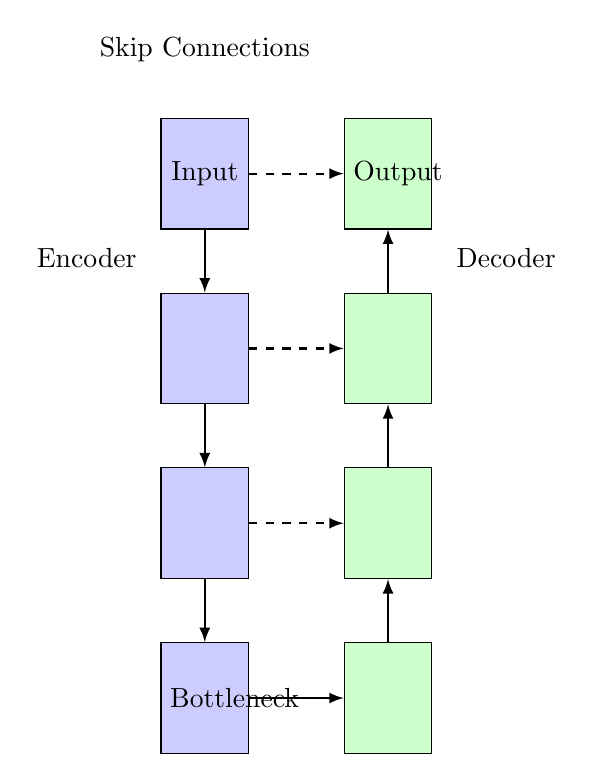
\begin{tikzpicture}[
    node distance=0.8cm and 1.2cm,
    block/.style={rectangle, draw, fill=blue!20, text width=2.5em, text centered, minimum height=4em},
    dblock/.style={rectangle, draw, fill=green!20, text width=2.5em, text centered, minimum height=4em},
    arrow/.style={-latex, thick}
]
    % Encoder Path
    \node[block] (e1) {Input};
    \node[block, below=of e1] (e2) {};
    \node[block, below=of e2] (e3) {};
    \node[block, below=of e3] (e4) {Bottleneck};

    % Decoder Path
    \node[dblock, right=of e4] (d4) {};
    \node[dblock, above=of d4] (d3) {};
    \node[dblock, above=of d3] (d2) {};
    \node[dblock, above=of d2] (d1) {Output};

    % Connections
    \draw[arrow] (e1) -- (e2);
    \draw[arrow] (e2) -- (e3);
    \draw[arrow] (e3) -- (e4);
    \draw[arrow] (e4) -- (d4);
    \draw[arrow] (d4) -- (d3);
    \draw[arrow] (d3) -- (d2);
    \draw[arrow] (d2) -- (d1);

    % Skip Connections
    \draw[arrow, dashed] (e3.east) to [out=0, in=180] (d3.west);
    \draw[arrow, dashed] (e2.east) to [out=0, in=180] (d2.west);
    \draw[arrow, dashed] (e1.east) to [out=0, in=180] (d1.west);
    
    % Labels
    \node[above=0.2cm of e2, xshift=-1.5cm, align=center] {Encoder};
    \node[above=0.2cm of d2, xshift=1.5cm, align=center] {Decoder};
    \node[above=0.1cm of d2, midway, yshift=1.2cm] {Skip Connections};

\end{tikzpicture}
\caption{A simplified diagram of the U-Net architecture, showing the symmetric encoder-decoder pathways and the skip connections that merge high-resolution features from the encoder with upsampled features in the decoder.}
\label{fig:unet_architecture}
\end{figure}


To further improve the quality of segmentation results, Conditional Random Fields (CRFs) are often used as a final refinement step after a CNN-based prediction. The use of CRFs helps to polish the initial pixel-level outputs, with a specific aim of creating sharper object boundaries and ensuring greater spatial coherence in the final segmentation map. These probabilistic models work by directly taking into account the spatial connections between adjacent pixels. This helps to reduce noise and ultimately leads to outputs that are not only more accurate but also more visually pleasing.

\section{Challenges and Future Directions}
\label{sec:challenges}

\subsection{Limited Training Data}
Despite significant advancements in data augmentation and transfer learning, the scarcity of labeled training data remains a critical obstacle for remote sensing image classification \cite{zhu2017deep}. The task of obtaining high-quality labels for remote sensing imagery is both costly and time-intensive, necessitating considerable manual work from experts in the field \cite{xia2017aid}.

To address this data shortage, self-supervised learning has surfaced as a highly promising approach. The main concept is to learn robust feature representations directly from extensive unlabeled datasets. This is done by creating "pretext" tasks, which could involve predicting image rotations, using contrastive learning goals, or filling in masked areas of an image. All these tasks motivate the model to acquire meaningful semantic features without the need for human-supplied labels.

In a similar context, weakly supervised and semi-supervised learning techniques provide another way to lessen the annotation workload \cite{zhang2016weakly}. These strategies are formulated to make use of more affordable and less exact types of supervision, like image-level tags or rough annotations. By skillfully blending a small, precisely labeled dataset with larger amounts of weakly labeled data, these methods can frequently deliver performance on par with fully supervised approaches, but at a much lower labeling expense.

\subsection{Computational Efficiency}
The growing scale and complexity of contemporary CNN models pose substantial challenges to their real-world application, particularly in environments with limited resources such as satellites or edge computing devices. Consequently, creating efficient model architectures and optimization methods is not merely advantageous but crucial for the broader implementation of these technologies in practical remote sensing scenarios.

To tackle this problem, a range of model compression methods has been formulated. These techniques, which encompass pruning, quantization, and knowledge distillation, are aimed at reducing the model's size and computational needs while attempting to preserve a high standard of performance. Such strategies operate by either systematically eliminating unnecessary parameters or by generating more condensed model versions, which in turn allows them to be used on platforms with restricted memory and processing capabilities.

Concurrently, neural architecture search (NAS) presents a more automated pathway to solve this issue. NAS algorithms are able to methodically search through a huge design space to find highly efficient network structures that are specifically tailored to certain hardware constraints and performance objectives. This automated design approach often leads to new architectural concepts that can exceed the performance of manually created models while also meeting strict computational budget requirements.

\subsection{Multi-modal Data Fusion}
Current remote sensing systems can acquire a rich variety of data from multiple sources, such as optical imagery, synthetic aperture radar (SAR), LiDAR, and hyperspectral sensors \cite{zhu2017deep}. Nevertheless, achieving an effective and synergistic combination of information from these different sources continues to be a major technical hurdle.

Early fusion represents the most direct class of strategies. These methods combine multi-modal data at the initial input stage, with a typical example being the simple concatenation of data from various sensors. Although straightforward in concept, these techniques require the precise spatial alignment of all data sources and can face difficulties when dealing with different spatial resolutions or when a specific data modality is unavailable.

On the other end of the methodological spectrum are late fusion techniques. In this approach, each data modality is processed on its own through a distinct network branch. The resulting predictions are then merged only at the final stage of decision-making. A significant benefit of this method is its natural resilience to missing modalities. However, a possible weakness is its inability to capture complex, low-level connections that might exist between the various data streams.

Intermediate fusion methods seek a compromise by aiming to merge features at different points within the network's structure. This approach enables a more complex and layered integration of multi-modal information. These more sophisticated techniques frequently use tools like attention mechanisms or specific cross-modal interaction layers to dynamically represent the intricate relationships between different data modalities. This process leads to a richer and more complete feature representation.

\subsection{Interpretability and Explainability}
The "black-box" nature of many deep learning models presents a considerable problem, especially in high-stakes remote sensing applications where understanding and trusting the model's decision-making process is crucial. As a result, the creation of interpretable and explainable AI methods has become a vital area of research for fostering confidence in and providing clarity for these complex systems.

Visualization techniques are a primary area of investigation. Methods like activation mapping, saliency maps, and class activation mapping are formulated to visually pinpoint which specific areas of an image have the greatest impact on the model's final output. By offering these windows into the model's internal processes, such techniques can supply important insights into its behavior and aid in identifying potential biases or points of failure.

It is noteworthy that attention mechanisms fulfill a dual role in this regard. Although they are frequently used to enhance model performance, they also provide a built-in form of interpretability. The attention weights can be displayed as a heatmap, which gives a clear visual cue as to where the model is "focusing" or what it is concentrating on when it arrives at a decision.

To achieve a more human-like understanding, concept-based explanation methods try to pinpoint the high-level, human-intelligible concepts that a model relies on to make its predictions. By closing the divide between abstract, low-level features and a vocabulary that people can easily understand, these methods can assist stakeholders in confirming that a model is in fact utilizing appropriate and logical features in its decision-making.

\begin{figure}[htbp]
\centering
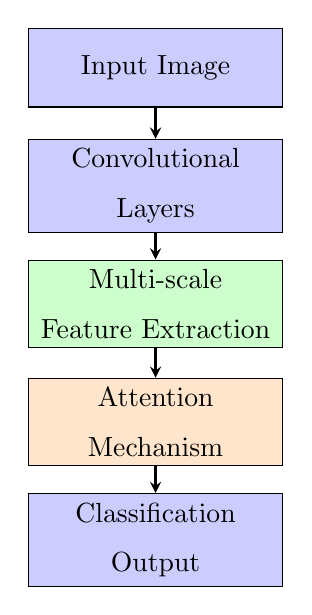
\begin{tikzpicture}[
    node distance=1.5cm,
    box/.style={rectangle, draw, fill=blue!20, text width=3cm, align=center, minimum height=1cm},
    arrow/.style={->, >=stealth, thick}
]
    % Input layer
    \node[box] (input) {Input Image};
    
    % Feature extraction
    \node[box, below of=input] (conv) {Convolutional Layers};
    
    % Multi-scale features
    \node[box, below of=conv, fill=green!20] (multiscale) {Multi-scale Feature Extraction};
    
    % Attention mechanism
    \node[box, below of=multiscale, fill=orange!20] (attention) {Attention Mechanism};
    
    % Classification
    \node[box, below of=attention] (output) {Classification Output};
    
    % Arrows
    \draw[arrow] (input) -- (conv);
    \draw[arrow] (conv) -- (multiscale);
    \draw[arrow] (multiscale) -- (attention);
    \draw[arrow] (attention) -- (output);
\end{tikzpicture}
\caption{General architecture of deep learning models for remote sensing image classification}
\label{fig:architecture}
\end{figure}

\section{Conclusion}
\label{sec:conclusion}

This review has provided a comprehensive survey of the recent and swift advancements in the use of deep learning for remote sensing image classification, placing a specific focus on innovations from the years 2020 to 2023. In the course of this review, we have examined key improvements in CNN architectures, new training strategies, and a variety of application-focused adaptations that have together driven substantial performance improvements across the discipline.

Our analysis highlights several important trends and significant breakthroughs. It is now evident that multi-scale feature extraction methods are essential for successfully managing the wide diversity of object sizes found in remote sensing imagery. In a similar vein, the use of attention mechanisms has shown to be a very effective approach for allowing models to concentrate on the most distinguishing regions and features in complex scenes. To address the ongoing problem of data scarcity, both transfer learning and domain adaptation techniques have been critically important. Moreover, the movement toward lightweight network architectures has been key in allowing these powerful models to be deployed on platforms with limited resources.

Nevertheless, despite this undeniable progress, a number of major challenges are still present. The accessibility of labeled training data, although improving, continues to be a significant limitation on performance. This is especially true for highly specialized tasks or for data originating from new sensor technologies. The demanding computational efficiency needs of many real-world environments also continue to create deployment difficulties. Moving forward, the methods for fusing multi-modal data need more development to realize the full potential of combining information from various sensor types. Finally, the vital questions of model interpretability and explainability remain a top priority, as establishing trust in the outputs of these intricate deep learning systems is a fundamental requirement for their broad acceptance and application.

\begin{table}[htbp]
\centering
\caption{Comparison of Deep Learning Approaches for Remote Sensing}
\label{tab:comparison}
\begin{tabular}{@{}llll@{}}
\toprule
\textbf{Method} & \textbf{Strength} & \textbf{Limitation} & \textbf{Best Use Case} \\ 
\midrule
CNN-based & High accuracy & Large data needed & Scene classification \\
Attention-based & Feature selection & Computational cost & Complex scenes \\
Lightweight & Efficiency & Lower accuracy & Edge deployment \\
Multi-modal & Rich information & Data alignment & Fusion tasks \\
\bottomrule
\end{tabular}
\end{table}

Looking forward, several areas of research seem particularly promising. Deeper investigation into self-supervised learning is vital for making better use of the extensive archives of unlabeled data. A sustained emphasis on creating efficient model designs is crucial for expanding the range of deployment on resource-limited devices. Additionally, there is a distinct requirement for more advanced techniques in multi-modal fusion and for more reliable methods that enhance model interpretability. Furthermore, the synergistic combination of modern deep learning with established remote sensing processing methods, along with the inclusion of specific domain knowledge, presents exciting possibilities for future innovations.

As the technology of remote sensing continues its swift progression, creating datasets that are ever more massive and complex, deep learning is set to assume an increasingly vital role in the process of deriving meaningful information and practical insights. For this reason, the ongoing and focused creation of specialized architectures and methods, designed specifically for the distinct challenges of remote sensing, will be absolutely fundamental for navigating the expanding opportunities and intricacies that characterize this vibrant field.


\bibliographystyle{IEEEtran}
\begin{thebibliography}{8}

\bibitem{zhu2017deep}
Zhu, X. X., Tuia, D., Mou, L., et al. (2017). Deep learning in remote sensing: A comprehensive review and list of resources. \emph{IEEE Geoscience and Remote Sensing Magazine}, 5(4), 8-36.

\bibitem{cheng2016survey}
Cheng, G., and Han, J. (2016). A survey on object detection in optical remote sensing images. \emph{ISPRS Journal of Photogrammetry and Remote Sensing}, 117, 11-28.

\bibitem{xia2017aid}
Xia, G. S., Hu, J., Hu, F., Shi, B., Bai, X., Zhong, Y., and Lu, X. (2017). AID: A benchmark data set for performance evaluation of aerial scene classification. \emph{IEEE Transactions on Geoscience and Remote Sensing}, 55(7), 3965-3981.

\bibitem{maggiori2017end}
Maggiori, E., Tarabalka, Y., Charpiat, G., and Alliez, P. (2017). Convolutional neural networks for large-scale remote-sensing image classification. \emph{IEEE Transactions on Geoscience and Remote Sensing}, 55(2), 645-657.

\bibitem{zhang2016weakly}
Zhang, F., Du, B., Zhang, L., and Xu, M. (2016). Weakly supervised learning based on coupled convolutional neural networks for aircraft detection. \emph{IEEE Transactions on Geoscience and Remote Sensing}, 54(9), 5553-5563.

\bibitem{liu2019learning}
Liu, Y., Chen, X., Wang, H., Ye, Z., Lin, Z., and Yu, P. S. (2019). Deep learning for pixel-level remote sensing data analysis: A review. \emph{ISPRS Journal of Photogrammetry and Remote Sensing}, 150, 1-15.

\bibitem{zeng2018improving}
Zeng, D., Chen, S., Chen, B., and Li, S. (2018). Improving remote sensing scene classification by integrating global-context and local-object features. \emph{Remote Sensing}, 10(7), 734.

\bibitem{deng2017enhanced}
Deng, Z., Sun, H., Zhou, S., Zhao, L., Lei, H., and Zou, H. (2017). Multi-scale object detection in remote sensing imagery with convolutional neural networks. \emph{ISPRS Journal of Photogrammetry and Remote Sensing}, 130, 83-94.

\end{thebibliography}

\end{document}